\documentclass[12pt]{article}

\usepackage[utf8]{inputenc}
\usepackage{amsmath,amsthm,amsfonts,amssymb,amscd}
\usepackage{multirow,booktabs}
\usepackage[table]{xcolor}
\usepackage{fullpage}
\usepackage{lastpage}
\usepackage{enumitem}
\usepackage{fancyhdr}
\usepackage{mathrsfs}
\usepackage{wrapfig}
\usepackage{setspace}
\usepackage{calc}
\usepackage{multicol}
\usepackage{cancel}

%%\usepackage[demo]{graphicx}
%%\usepackage{caption}
%%\usepackage{subcaption}


\usepackage{listings}
\usepackage{matlab-prettifier}
\usepackage[framed,numbered,autolinebreaks,useliterate]{mcode}

\usepackage[margin=3cm]{geometry}
\newlength{\tabcont}
\setlength{\parindent}{0.0in}
\setlength{\parskip}{0.05in}
\usepackage{empheq}
\usepackage{framed}
\usepackage[most]{tcolorbox}
\usepackage{xcolor}
\colorlet{shadecolor}{orange!15}
\parindent 0in
\parskip 12pt
\geometry{margin=1in, headsep=0.25in}
\usepackage{float}
\usepackage{graphicx}
\usepackage{hyperref}


\newtheorem{thm}{Theorem}
\theoremstyle{theorem}
\newtheorem{reg}{Rule}
\newtheorem{exe}{Exercise}
\newtheorem{rem}{Remark}
\newtheorem{cor}{Corollary}
\newtheorem{exa}{Example}

\usepackage{natbib}
\bibliographystyle{abbrv}

\usepackage{times}

%\usepackage[compact]{titlesec}
\usepackage{titlesec}
\titlespacing*{\section}{0pt}{*-2}{*-1}
\titlespacing*{\subsection}{0pt}{*-2}{*-1}

\def\a{\alpha}
\def\b{\beta}
\def\de{\delta}
\def\De{\Delta}
\def\ga{\gamma}
\def\Si{\Sigma}
\def\si{\sigma}
\def\ep{\varepsilon}
\def\ze{\zeta}
\def\om{\omega}
\def\leq{\leqslant}
\def\rar{\rightarrow}
\def\Rar{\Rightarrow}
\def\td{\Leftrightarrow}
\def\R{\hro{R}}
\def\C{\hro{C}}
\def\hro{\mathbb}
\def\bbI{\hro{I}}
\def\N{\hro{N}}
\def\Z{\hro{Z}}

\def\tE{\tilde{E}}
\def\hE{\hat{E}}
\def\tA{\tilde{A}}
\def\tT{\tilde{T}}
\def\hA{\hat{A}}
\def\hD{\hat{D}}
\def\bA{\breve{A}}
\def\tB{\tilde{B}}
\def\hB{\hat{B}}
\def\tC{\tilde{C}}
\def\tN{\tilde{N}}
\def\hN{\hat{N}}
\def\tk{\tilde{k}}
\def\tX{\tilde{X}}
\def\hX{\hat{X}}
\def\bX{\breve{X}}
\def\tM{\tilde{M}}
\def\tm{\tilde{m}}
\def\bM{\breve{M}}
\def\hM{\hat{M}}
\def\bm{\breve{m}}
\def\tH{\tilde{H}}
\def\tF{\tilde{F}}
\def\tG{\tilde{G}}
\def\hG{\hat{G}}
\def\tK{\tilde{K}}
\def\tx{\tilde{x}}
\def\tf{\tilde{f}}
\def\hf{\hat{f}}
\def\brf{\breve{f}}
\def\baf{\bar{f}}
\def\tg{\tilde{g}}
\def\hg{\hat{g}}
\def\lb{\lambda}
\def\cP{{\cal P}}
\def\cQ{{\cal Q}}
\def\fr{\frac}
\def\frQ{\mathfrak{Q}}

\def\cU{{\cal U}}
\def\cV{{\cal V}}
\def\cH{{\cal H}}
\def\tcU{{\tilde{\cal U}}}
\def\cZ{{\cal Z}}

\def\hxi{\widehat{\xi}}
\def\hp{\hat{q}}

\def\ddt{\fr{\mathrm{d}}{\mathrm{d}t}}
\def\dtau{\Delta_{\tau}}
\def\tnu{\tilde{\nu}}
\def\tU{\tilde{U}}

\def\tcQ{{\tilde{\cal Q}}}
\def\tcP{{\tilde{\cal P}}}
\def\hcP{\widehat{\cP}}
\def\hcQ{\widehat{\cQ}}
\def\cE{\mathcal{E}}
\def\cA{\mathcal{A}}
\def\cD{\mathcal{D}}
\def\hcE{\hat{\cE}}
\def\hcA{\hat{\cA}}
\def\hcD{\hat{\cD}}
\def\vphi{\varphi}

\newcommand{\n}[1]{\left\lVert#1\right\rVert}

\newcommand{\m}[1]{
	\begin{bmatrix}
		#1
	\end{bmatrix}
}

\renewcommand{\pm}[1]{
	\begin{matrix}
		#1
	\end{matrix}
}

\def\ES{
	\begin{bmatrix}
		J^E  & 0        & 0       & 0 \\
		0       & N^E_{2} & 0       & 0 \\
		0       & 0        & N^E_{3}& 0 \\
		0       & 0        & 0       & N^E_{4} 
	\end{bmatrix}
}

\def\AS{
	\begin{bmatrix}
		A_{1}  & 0       & 0          &  0        \\
		0           & J^A  & 0          & 0      \\
		0           &   0                & N^A_{3}      & 0      \\
		0           &   0                & 0                    & N^A_{4}      
	\end{bmatrix}
}
\def\BS{
	\begin{bmatrix}
		B_{1}  & 0       & 0        & 0 \\
		0          & B_{2}       & 0        & 0 \\
		0          & 0                  & J^B  & 0  \\
		0          & 0                 &   0                & N^B_{4}  \\ 
	\end{bmatrix}
}

\def\be{\begin{equation}}
\def\ee{\end{equation}}         

\newcommand{\ben}{\begin{eqnarray}}
\newcommand{\een}{\end{eqnarray}}

\newcommand{\bens}{\begin{eqnarray*}}
\newcommand{\eens}{\end{eqnarray*}}

\def\bc{\begin{cases}}
\def\ec{\end{cases}}

\newcommand{\bsq}{\begin{subequations}}
\newcommand{\esq}{\end{subequations}}

\newcommand{\eproof}{\space
	{\ \vbox{\hrule\hbox{\vrule height1.3ex\hskip0.8ex\vrule}\hrule}}\\[0.2cm]}

\begin{document}
% \setcounter{section}{8} This is assumed that count from Section 9
\thispagestyle{empty}

\begin{center}
	{\LARGE \bf Chapter 3 Rootfinding}\\[.2cm]
	{\large Numerical Analysis 1. Winter Semester 2018-19}
\end{center}

\section{Bisection Method}

\subsection{Matlab code}
The procedure to be constructed will operate on an arbitrary function f . An interval $[a, b]$ is also specified, and the number of steps to be taken, nmax, is given. Pseudocode to perform nmax steps in the bisection algorithm follows:

\begin{shaded}
 \lstinputlisting[language=Matlab]{Matlab_codes/bisection.m}
\end{shaded}

\subsection{Error bound}

\begin{figure}[h!]
	\centering
	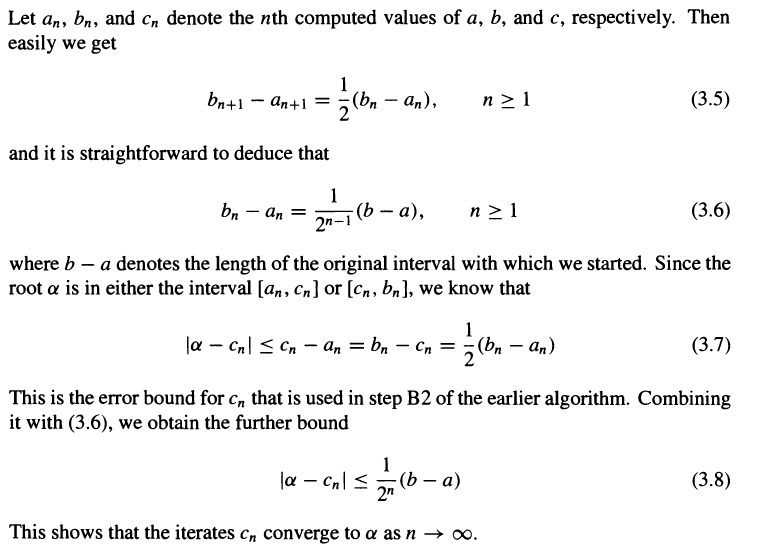
\includegraphics[width=0.99\linewidth]{Figures/screenshot002}
	\caption{Atkinson-Han, page 74}
	\label{fig:screenshot002}
\end{figure}

\pagebreak 

\begin{figure}[h!]
	\centering
	
\includegraphics[scale=0.8]{Figures/screenshot003}
	%\caption{Atkinson-Han, page 74}
	\label{fig:screenshot002}
\end{figure}

Thus we have the following estimation 
%
\begin{shaded}
\be\label{error bound}
 n \geq \cfrac{ \log \big( \cfrac{b-a}{\epsilon} \big) }{ \log 2 } \quad .
\ee 
\end{shaded}
%
There are several advantages to the bisection method. The principal one is that the method is guaranteed to converge. In addition, the error bound, given in (3.7), is guaranteed to decrease by one-half with each iteration. Many other numerical methods have variable rates of decrease for the error, and these may be worse than the bisection method for some equations. The principal disadvantage of the bisection method is that it generally converges more slowly than most other methods. For functions $f(x)$ that have a continuous derivative, other methods are usually faster. These methods may not always converge; when they do converge, however, they are almost always much faster than the bisection method. 

\begin{rem}
As a final remark, to determine which subinterval of [an, bn] contains a root of f, it is better to make use of the signum function, since 
the test
%
\[ \mathrm{sign} (f(a_n)) \cdot \mathrm{sign}(f(c_n)) > 0 \mbox{ instead of } f(a_n) \cdot f(c_n) > 0 \]
%
gives the same result but avoids the possibility of overflow or underflow in the multiplication of $f(a_n)$ and $f(c_n)$.
\end{rem}

\pagebreak 

\section{Fix point iteration}
In this section, we give a more general introduction to iteration methods, presenting a general theory for one-point iteration formulas. 

\subsection{Classical fixed point iteration}

\begin{figure}[h!]
\centering
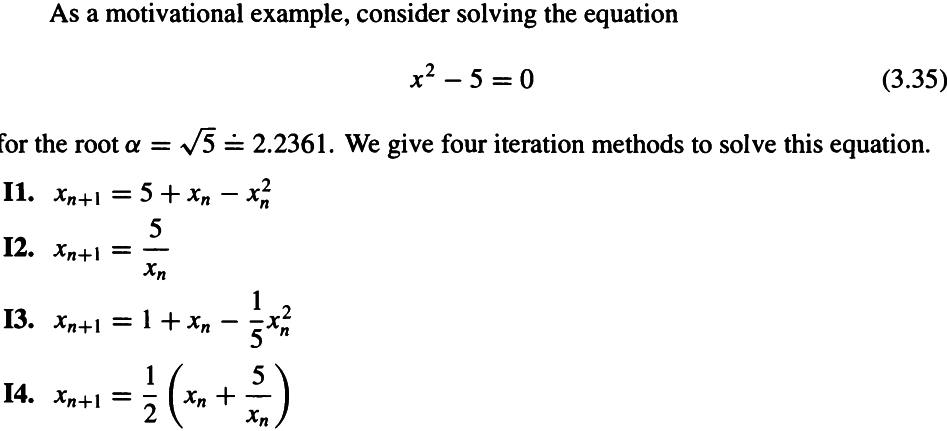
\includegraphics[scale=0.55]{Figures/screenshot005}
%\caption{Page 97 Atkinson - Han}
\label{fig:screenshot005}
\end{figure}

\begin{figure}[h!]
	\centering
	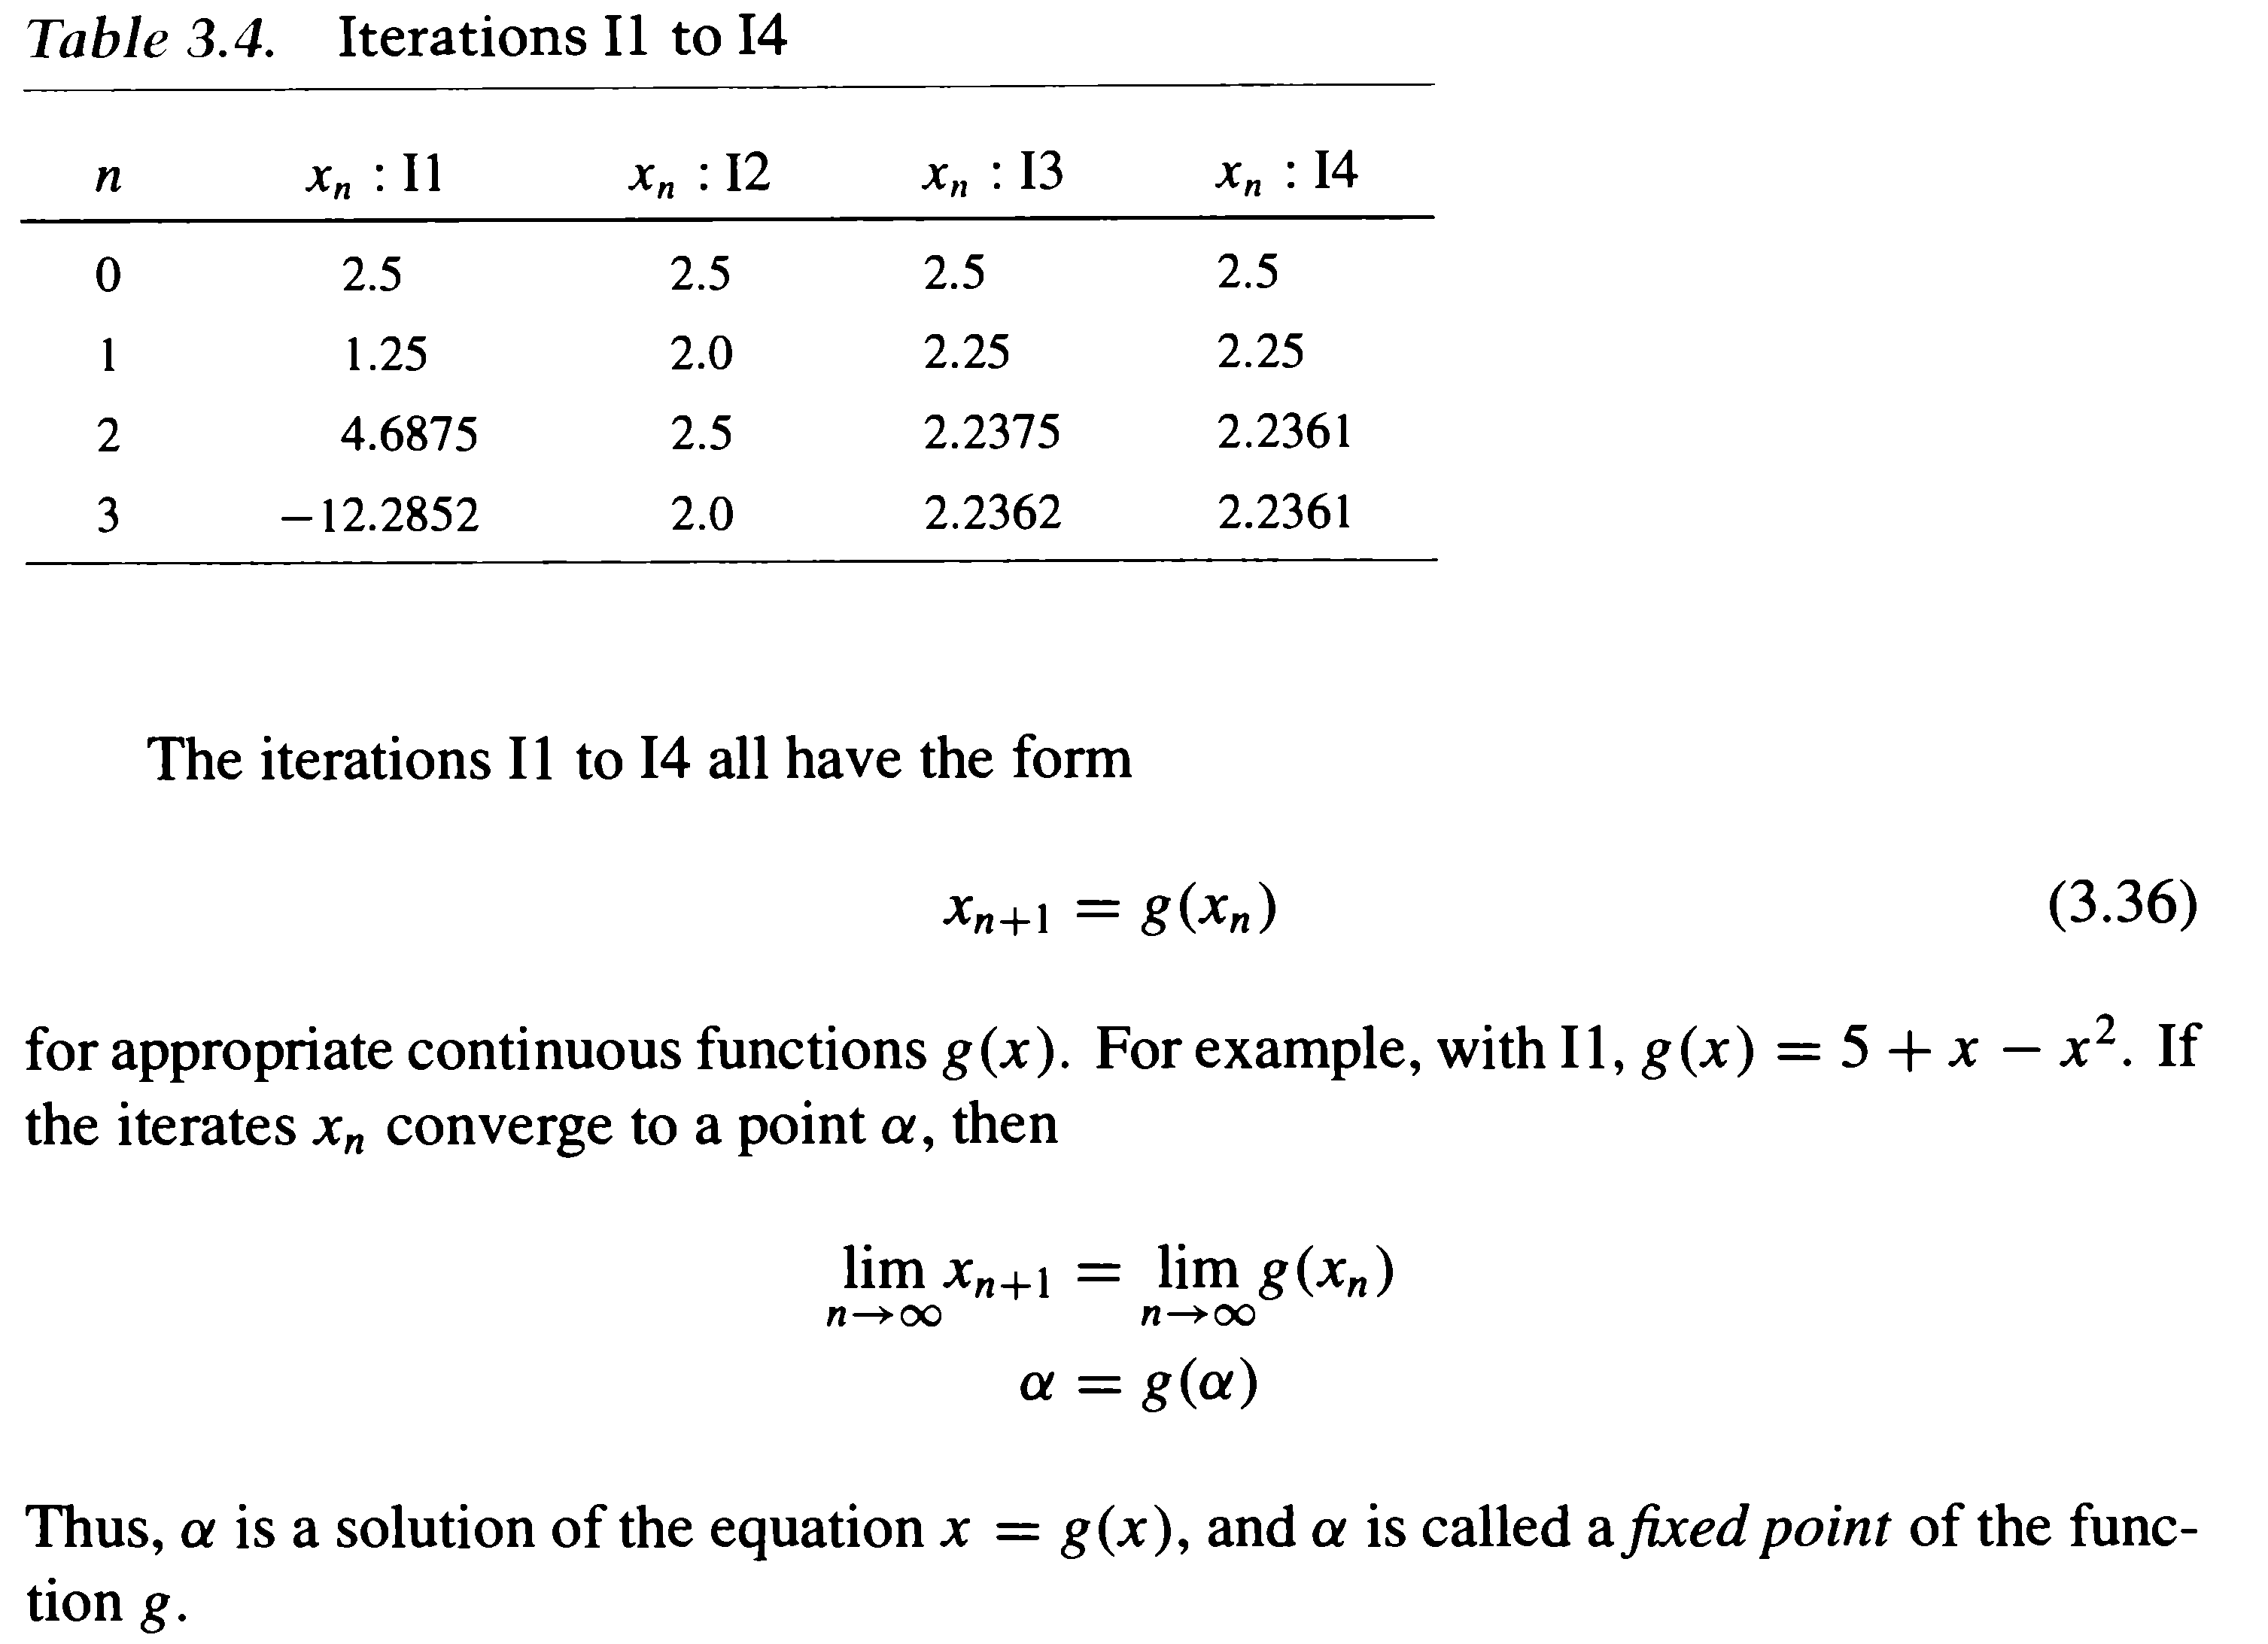
\includegraphics[scale=1.1]{Figures/screenshot006}
	\caption{Page 97 Atkinson - Han}
	\label{fig:screenshot005}
\end{figure}


\begin{shaded}
\begin{thm}\label{thm1} (Contraction mapping theorem) \\
Assume $g(x)$ and $g'(x)$ are continuous function and assume $g$ satisfies $g:[a,b] \rightarrow [a,b]$. Further assume that 
%
\[  \lb \equiv \underset{t\in [a,b]}{\max} |g'(x)| < 1. \]
%
Then
\begin{enumerate}
\item[S1.] There is a unique solution of $x = g(x)$ in the interval $[a, b]$ and for any initial estimate $x_0$ in $[a, b]$, the iterates $x_n$ will converge to $\a$. 
\item[S2.] \textbf{Priori error estimation}
%
\begin{equation}\label{pri}
  |\a-x_n| \leq \cfrac{\lb^n}{1-\lb} |x_1-x_0| \ . 
\end{equation}
%
\item[S3.] \textbf{Posteriori error estimation}
%
\begin{equation}\label{post}
 |\a-x_n| \leq \cfrac{\lb}{1-\lb} |x_{n}-x_{n-1}| \ .
\end{equation}
%
\item[S4.] 
%
\[ \underset{n\rar \infty}{\lim} \cfrac{\a - x_{n+1}}{\a-x_n} = g'(\a) \ .\]
%
Thus, 
%
\begin{equation}\label{eq1}
 |\a - x_{n+1}| \approx g'(\a) |\a - x_{n}| \ . 
\end{equation} 
%
\end{enumerate}	
\end{thm}
\end{shaded}
\begin{proof} The proof is taken from Atkinson-Han, \cite{AtkH03}.
\end{proof}
\begin{figure}[h!]
	\centering
	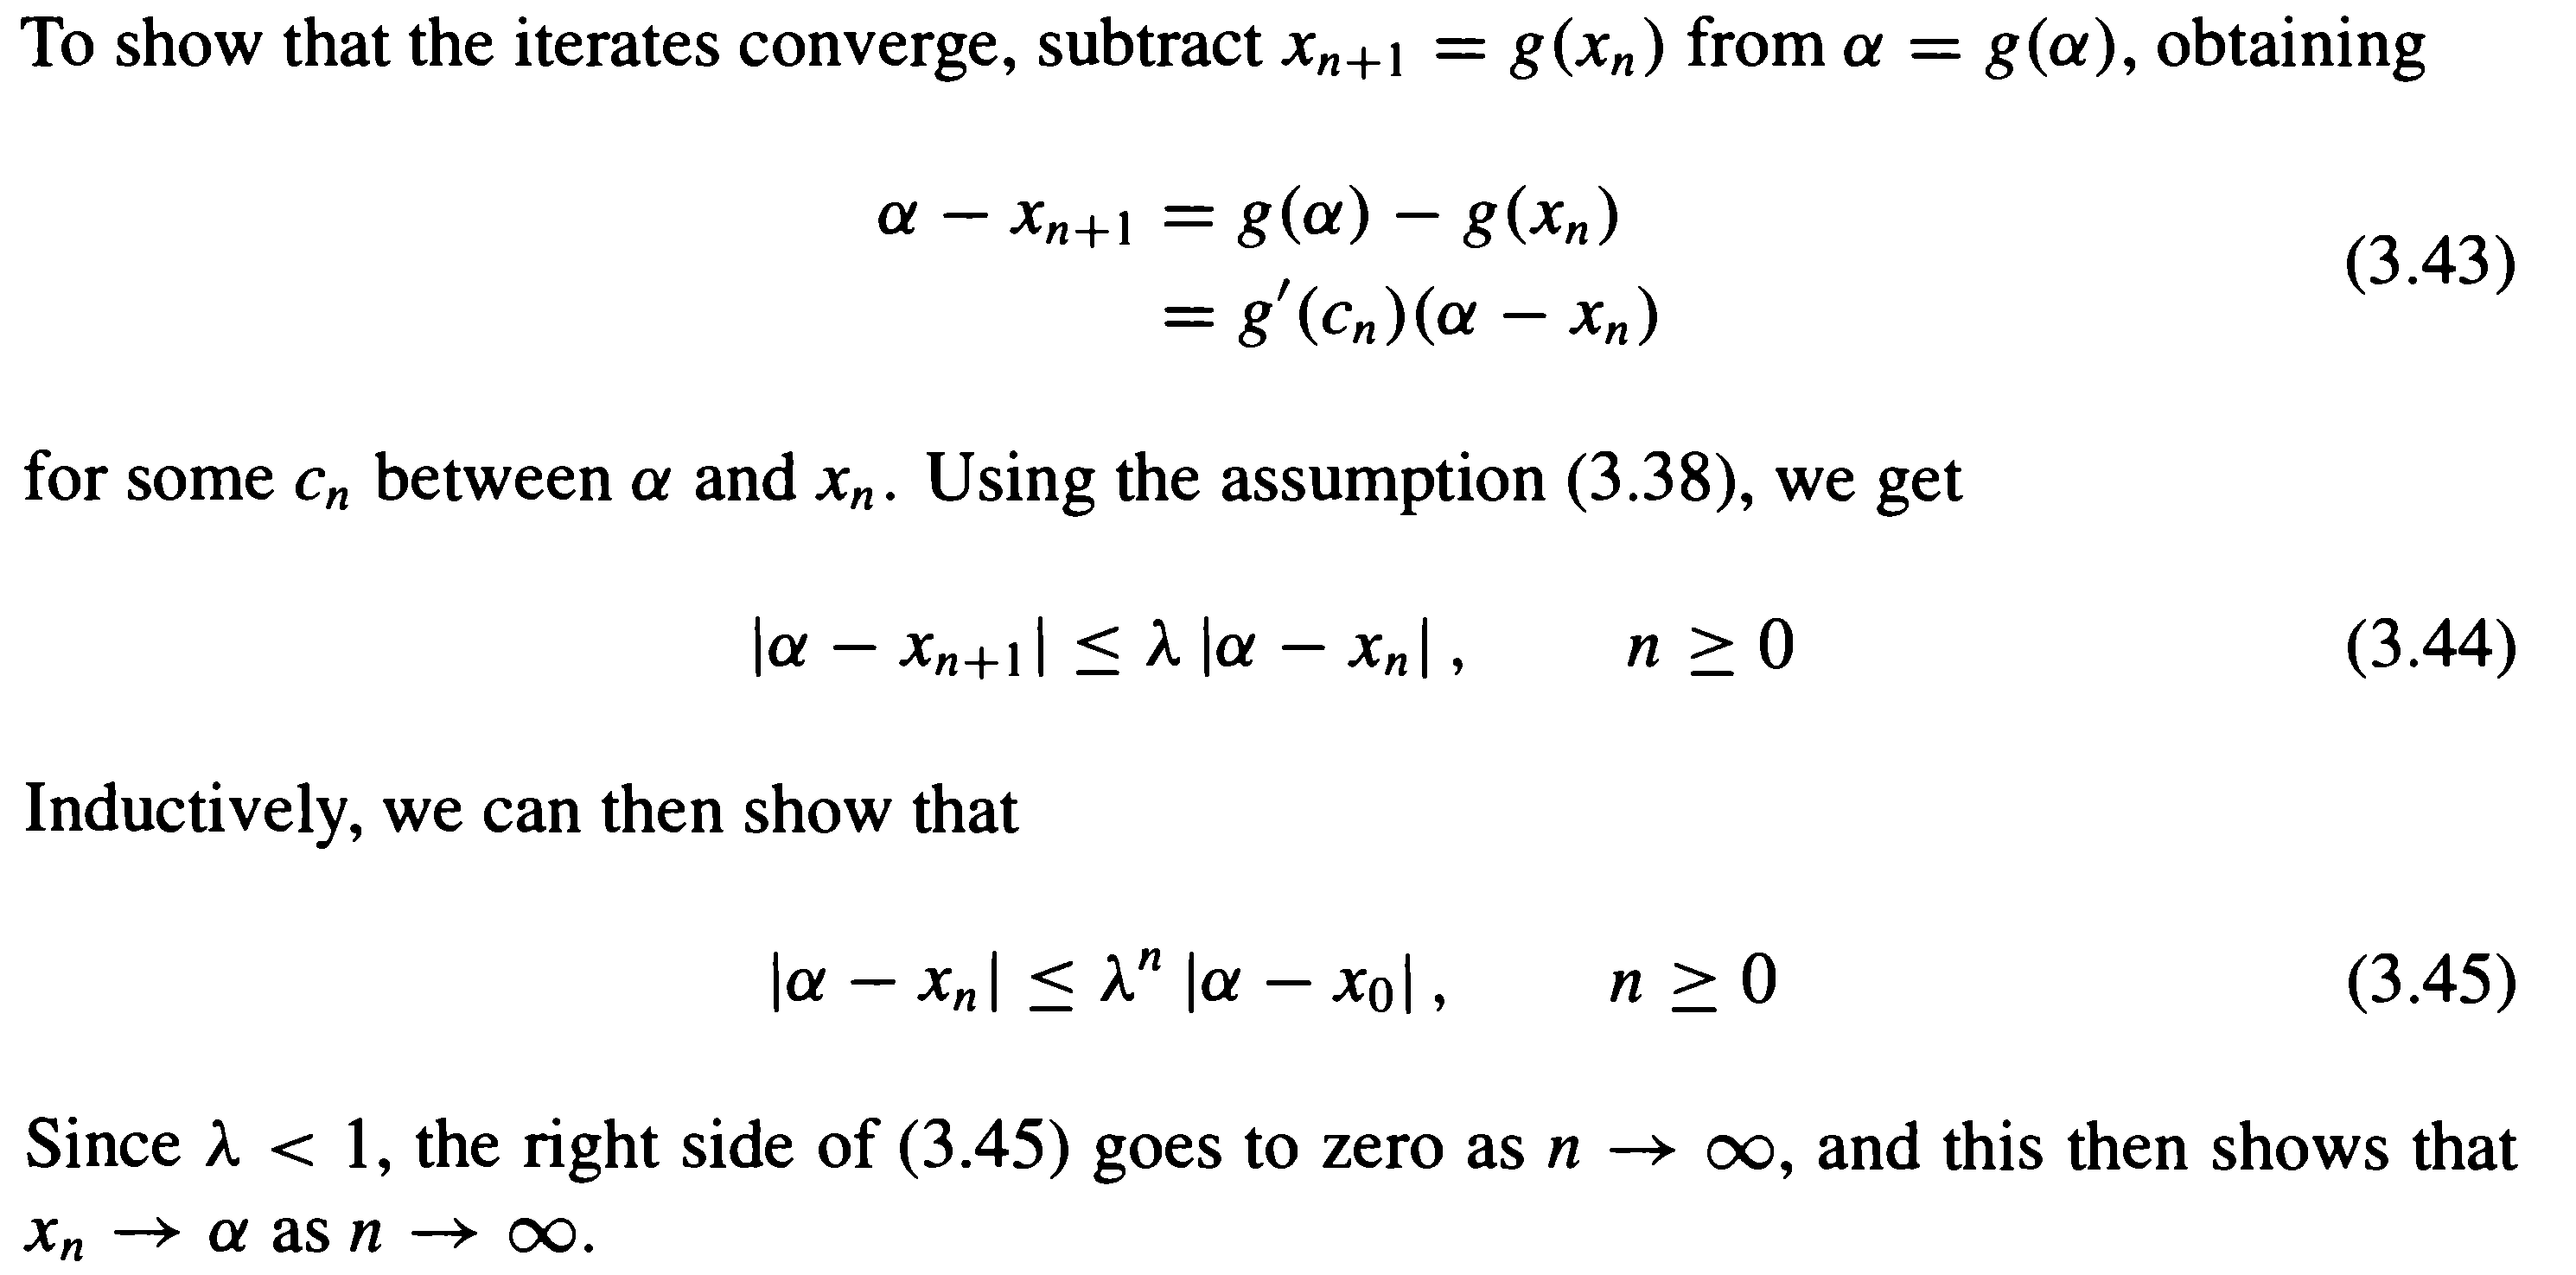
\includegraphics[scale=1.1]{Figures/screenshot007}
	%\caption{AtkinsonHan p100}
	\label{fig:screenshot007}
	\end{figure}
	
	\begin{figure}[h!]
		\centering
		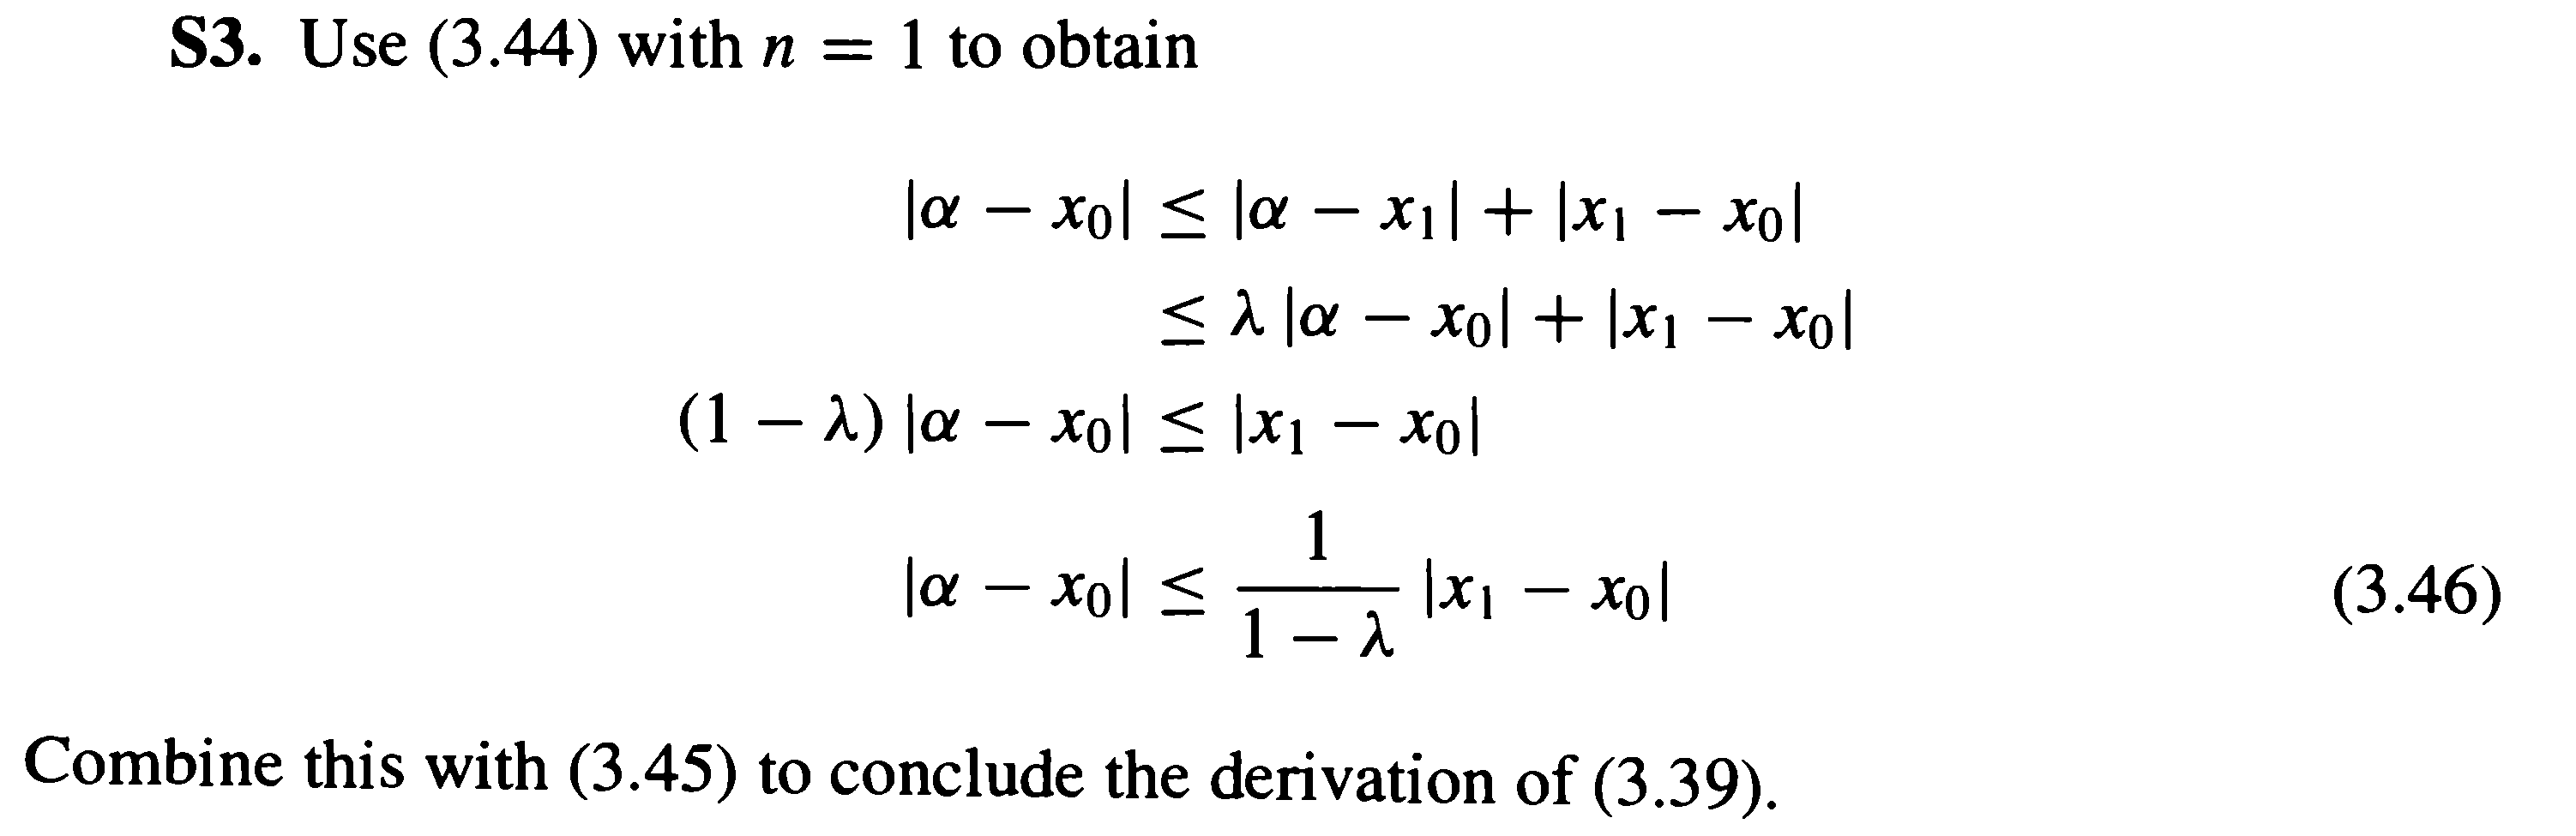
\includegraphics[scale=1.1]{Figures/screenshot008}
		\caption{AtkinsonHan p100}
		\label{fig:screenshot007}
		\end{figure}

\begin{shaded}
\begin{rem}
i) With the priori error estimation, we can compute the number of iteration needed to achieve a desired error $\ep$ without computing the approximated solution.\\
ii) On the other hand, the posteriori error estimation is convenient for computing, since if the absolute error between two consecutive error 
$|x_{n+1}-x_n|<\cfrac{\ep (1-\lb)}{\lb}$ then $|x_n-\a|<\ep$.\\
iii) The approx. \eqref{eq1} is useful for later.
\end{rem}
\end{shaded}
%
\begin{figure}[h!]
\centering
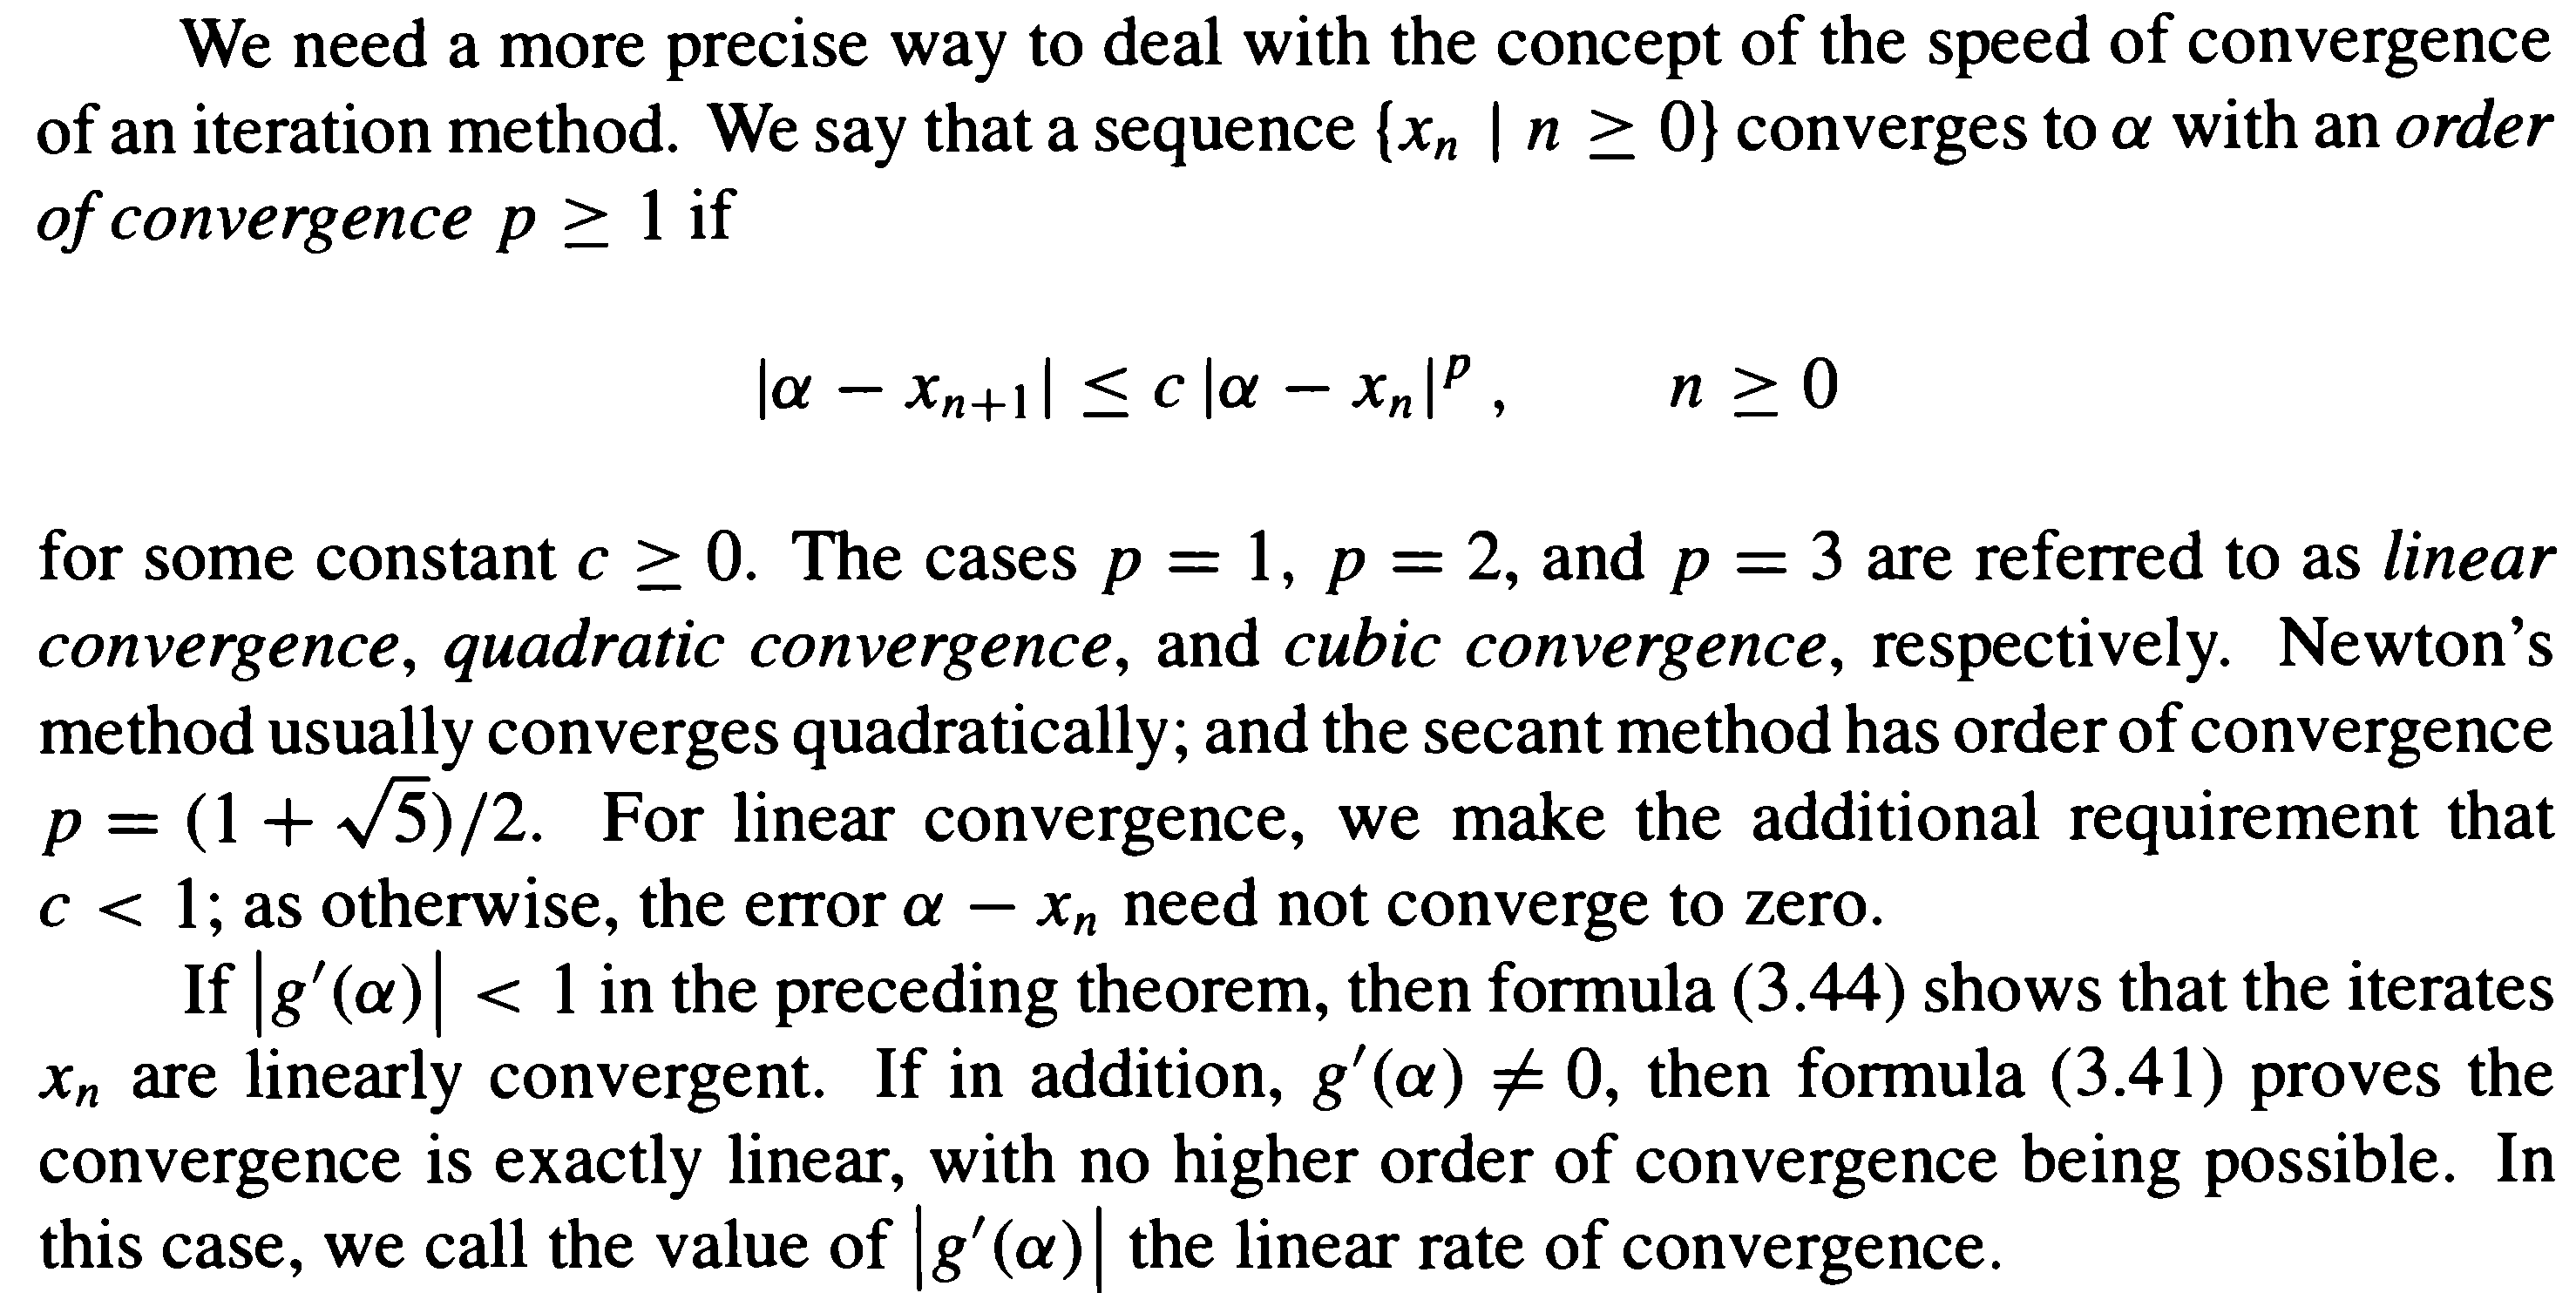
\includegraphics[scale=1.2]{Figures/screenshot009}
\caption{AtkinsonHan - very important}
\label{fig:screenshot009}
\end{figure}
%
In practice, Theorem \ref{thm1} is seldom used directly. The main reason is that it is difficult to find an interval $[a,b]$ for which the condition $g:[a,b] \rightarrow [a,b]$ is satisfied. Instead, we look for a way to use the theorem in a practical way. The key idea is the result \eqref{eq1}, which shows how the iteration error behaves when the iterates $x_n$ are near $\a$. 

\begin{shaded}
\begin{cor}
i) Assume that $g(x)$ and $g’(x$) are continuous for some interval $c<x<d$, with the fixed point ($\a$ contained in this interval. Moreover, assume that $|g'(a)| < 1$. Then, there is an interval $[a, b]$ around $\a$ for which the hypotheses, and hence also the conclusions, of Theorem \ref{thm1} are true. \\
ii) If the contrary, $|g'(\a)| > 1$, then the iteration method $x_{n+1} = g(x_n)$ will not converge to $\a$. \\
iii) When $|g'(\a)| = 1$, no conclusion can be drawn; and even if convergence were to occur, the method would be far too slow for the iteration method to be practical.
\end{cor}
\end{shaded}

Other remarks can be found in \cite{PKA}, pages 139, 141.

\subsection{Aitken Error Estimation and Extrapolation}
With the formula \eqref{eq1}, it is possible estimate the error in the iterate $x_n$ and to accelerate their convergence.
Let $g'(\a)$ be denoted by $\lb$. Thus,
%
\begin{equation}\label{eq2}
|\a - x_{n+1}| \approx \lb |\a - x_{n}| \ \Rightarrow \ \a \approx x_n + \cfrac{\lb}{1-\lb} \ (x_n-x_{n-1}). 
\end{equation} 
%
We need an estimate of $\lb$. It cannot be calculated from its definition, since that requires knowing the solution $\a$. To estimate $\lb$, we use the ratios
%
\begin{equation}
 \lb_n := \cfrac{x_n-x_{n-1}}{x_{n-1}-x_{n-2}} = g'(c_n) \overset{n\rar \infty}{\longrightarrow} g'(\a) = \lb \ .
\end{equation}
%
The \textbf{Aitken's extrapolation formula}
%
\[ \a \approx x_n + \cfrac{\lb_n}{1-\lb_n} \ (x_n-x_{n-1}) \  = \cfrac{x_{n-2} x_n - x_{n-1}^2}{x_{n-2} - 2 x_{n-1} + x_n}.  \]
%
The \textbf{Aitken's error estimate}
%
\[ \a - x_n \approx \cfrac{\lb_n}{1-\lb_n} \ (x_n-x_{n-1}) \  = \cfrac{ (x_n - x_{n-1})^2}{x_{n-2} - 2 x_{n-1} + x_n}.  \]
%

\begin{figure}[H]
\centering
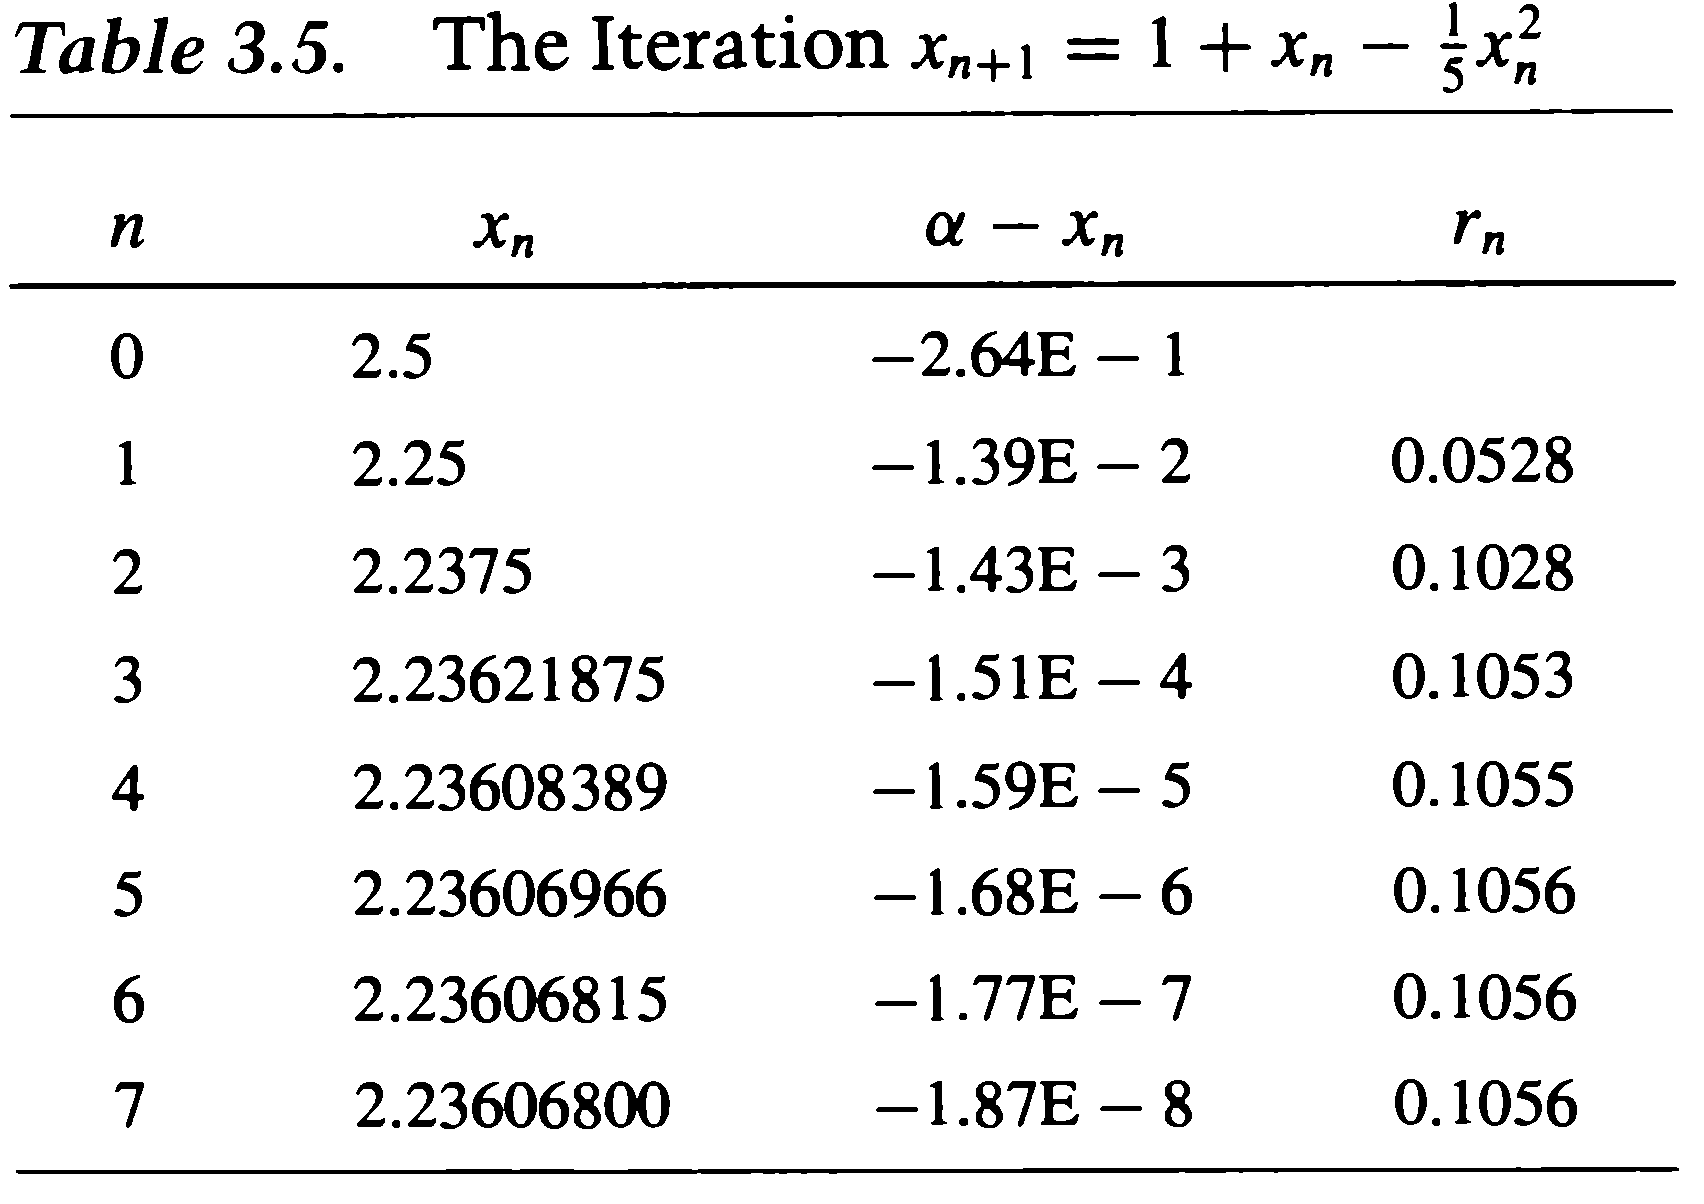
\includegraphics[scale=1.0]{Figures/screenshot0010}
\label{fig:screenshot0010}
\end{figure}

\begin{figure}[H]
\centering
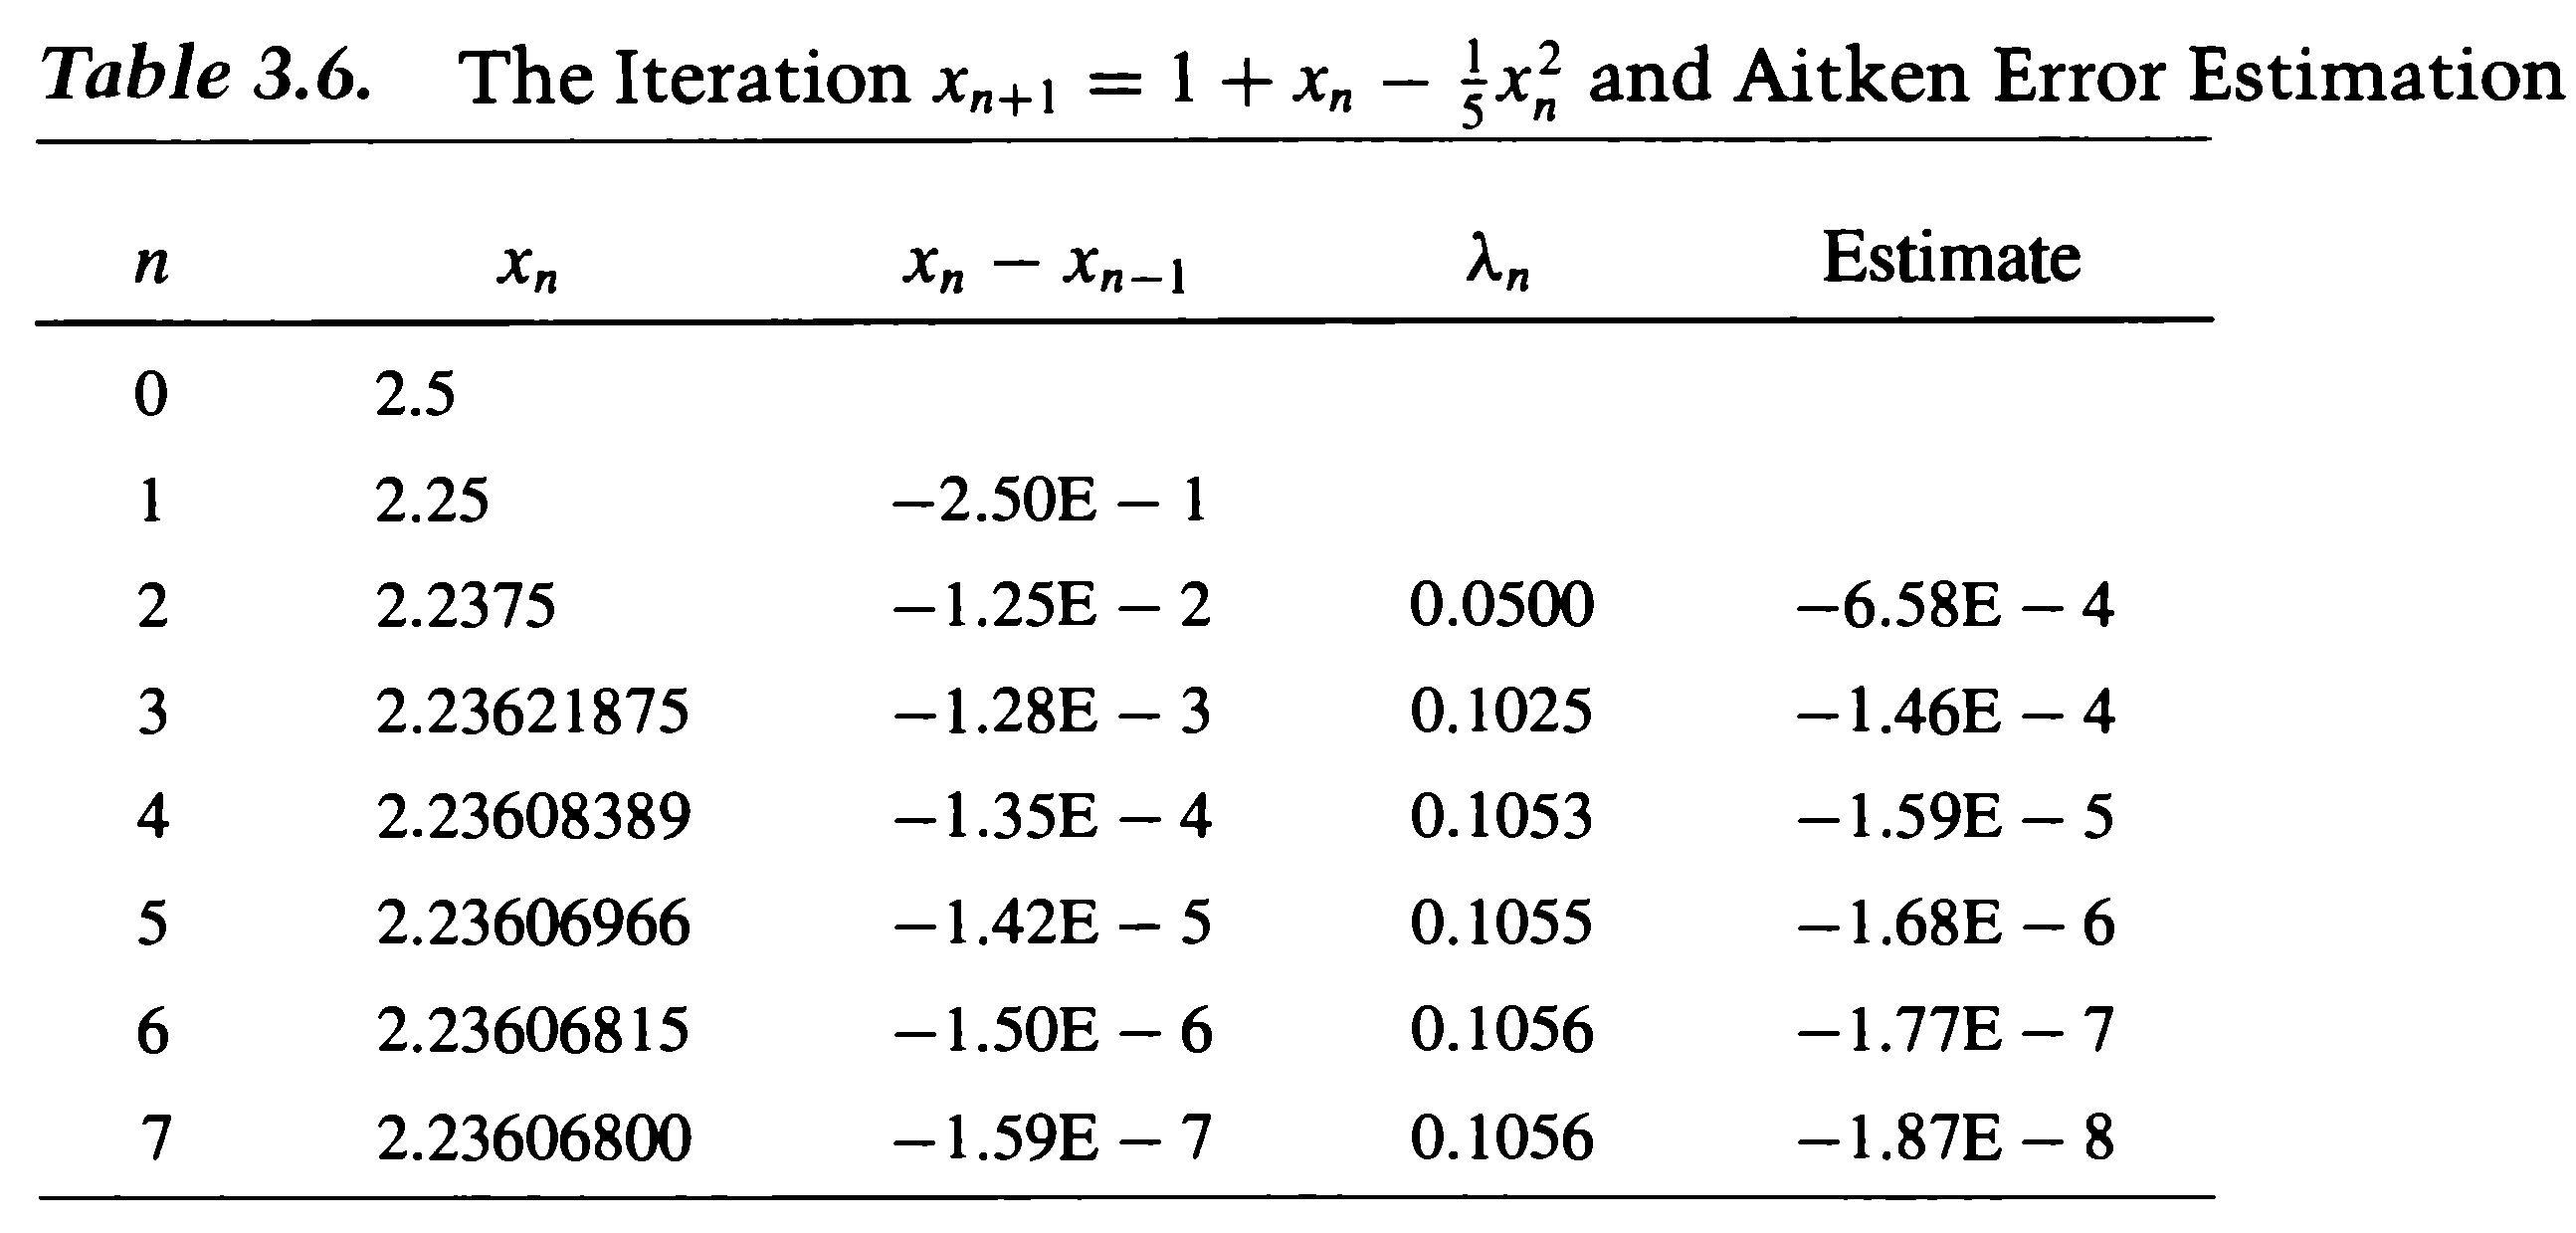
\includegraphics[scale=1.0]{Figures/screenshot0011}
\label{fig:screenshot0011}
\end{figure}

\subsection{Matlab code}
\begin{shaded}
	\lstinputlisting[language=Matlab]{"Matlab_codes/fix_iter.m"}
\end{shaded}

\subsection{Higher order iteration formulas}

\begin{figure}[H]
\centering
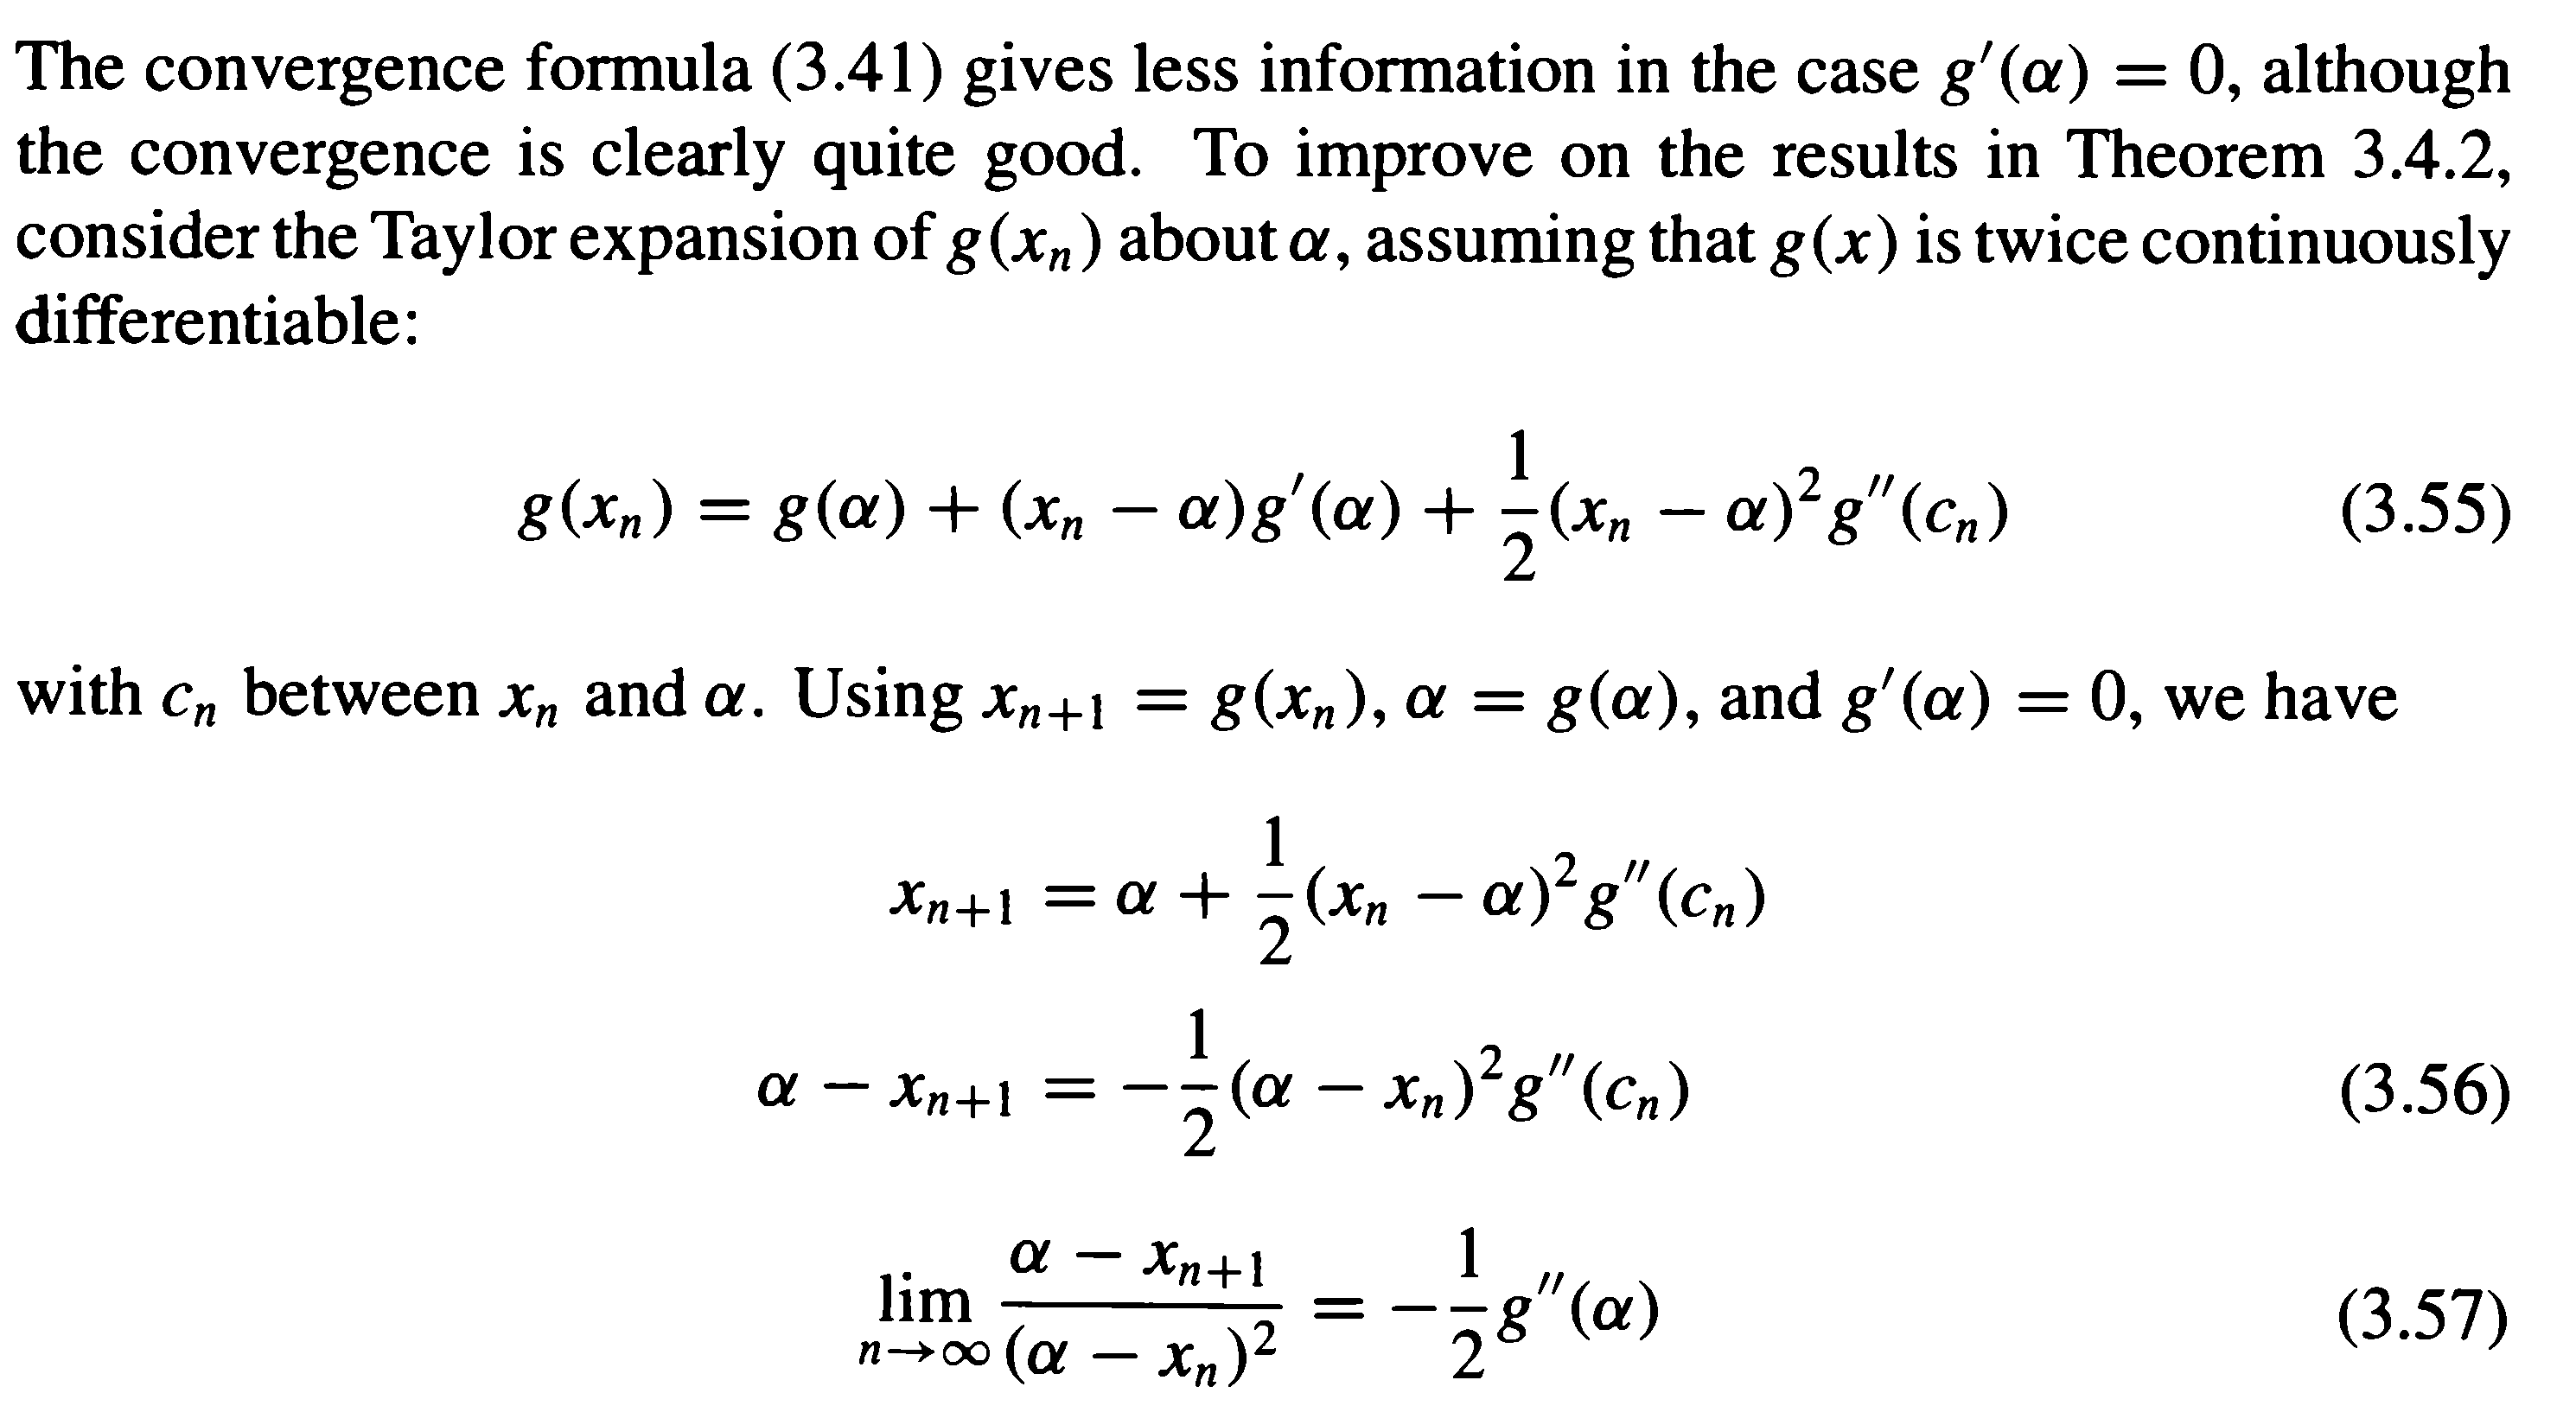
\includegraphics[scale=1.0]{Figures/screenshot0012}
\label{fig:screenshot0012}
\end{figure}

\begin{figure}[h!]
\centering
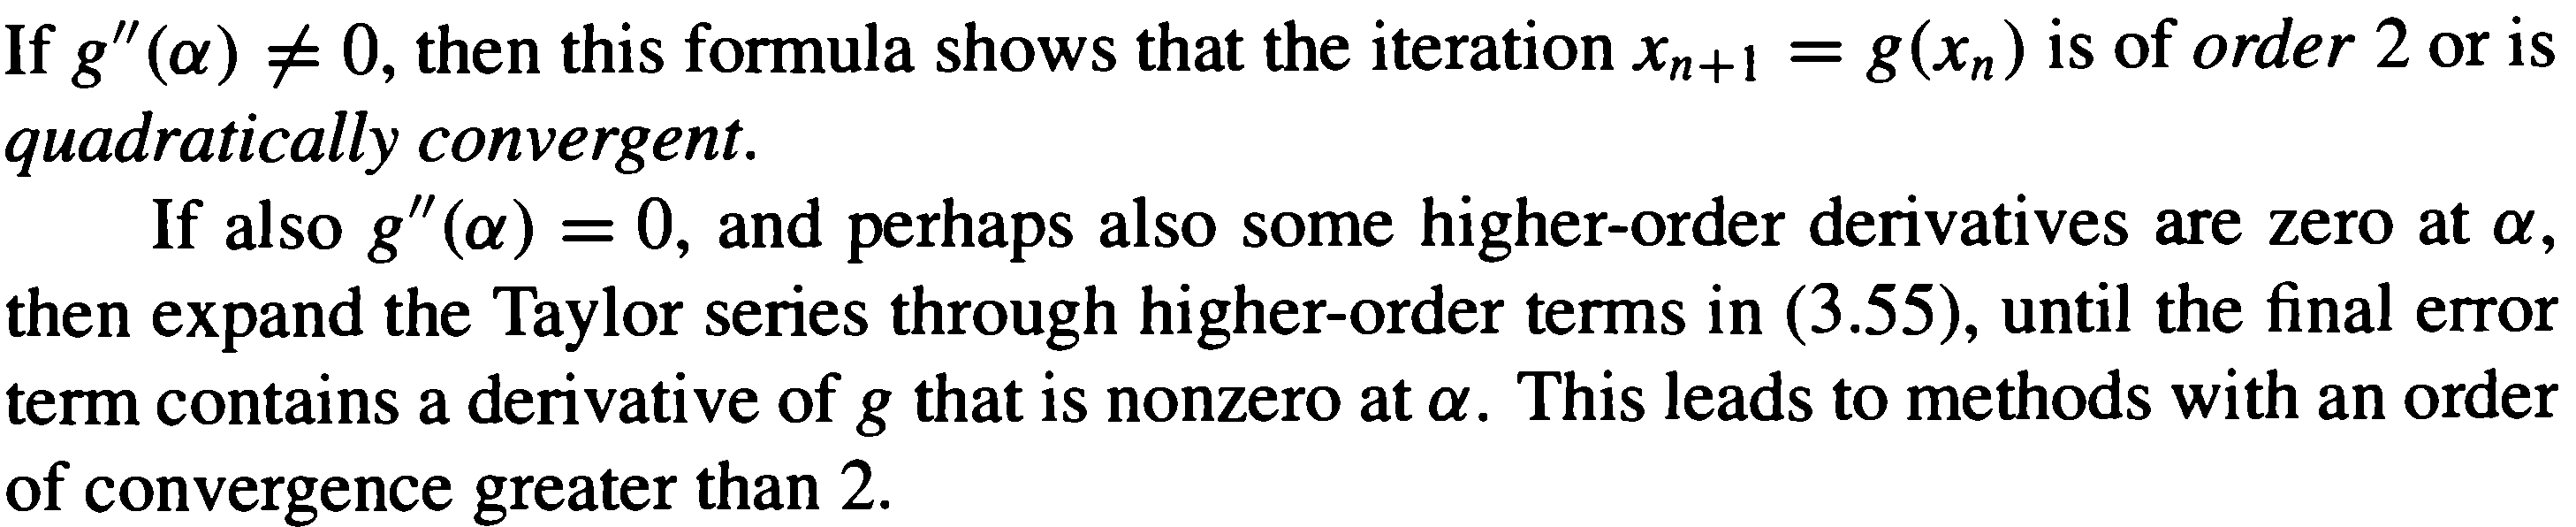
\includegraphics[scale=1.0]{Figures/screenshot0013}
\label{fig:screenshot0013}
\end{figure}

\cleardoublepage

\section{Newton method}

There are two ways to interpret the Newton (also named Newton-Raphson) method. 
\begin{enumerate}
\item[1.]  \textbf{Geometrical way}
\begin{figure}[h!]
\begin{minipage}{.5\textwidth}
	\centering
    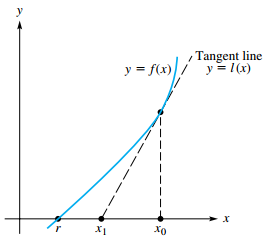
\includegraphics[scale=0.8]{Figures/screenshot0015}
    \caption{Newton method}
    \label{fig:screenshot0015}    
\end{minipage}%
\begin{minipage}{0.5\textwidth}
The \textbf{Newton method} reads	
\begin{framed}
%
\[  x_{n+1} = x_n - \cfrac{f(x_n)}{f'(x_n)} \ .	\]
%
\end{framed}
The geometry of Newton’s method is shown in Figure \ref{fig:screenshot0015}. The line $y = \ell(x)$ is tangent to the curve $y =f(x)$. It intersects the $x$-axis at a point $x_1$. The slope of $\ell(x)$ is $f'(x_0)$.  
\end{minipage}
\end{figure}    
\item[2.] \textbf{Analytical way}
We ask: What correction h should be added to $x_0$ to obtain the root precisely? Obviously, we want $f(x_0 + h) = 0$. If f is a sufficiently well-behaved function, it will have a Taylor series at $x_0$. Thus, we could write \\
%
\[ f(x_0) + h f'(x_0) + h^2 \cfrac{f"(x_0)}{2!} + \dots = 0 \ . \]
%
Determining $h$ from this equation is, of course, not easy. Therefore, we give up the expectation of arriving at the true root in one step and seek only an approximation to $h$. This can be obtained by ignoring all but the first two terms in the series: \ $f(x_0) + h f'(x_0) = 0$. 
The $h$ that solves this is not the $h$ that solves $f(x_0 + h) = 0$, but it is the easily computed number \& our new approximation is then
%
\[  x_{1} = x_0 - \cfrac{f(x_0)}{f'(x_0)} \ .	\]
%
and the process can be repeated. \\
This analytical way makes sense also in the case of systems of nonlinear equations, and we then have the Newton iterations
\begin{framed}
%
\[ \mathbf{ X_{n+1} = X_n - J_f(X_n)^{-1} F(X_n) \ \overset{MATLAB}{=}  X_n - J_f(X_n) \setminus F(X_n).) } \]
%
\end{framed}
\end{enumerate}

\subsection{Matlab code}

\begin{shaded}
	\lstinputlisting[language=Matlab]{Matlab_codes/newton.m}
\end{shaded}

\subsection{Experiments and Error analysis}

\begin{exa}
Example 3.2.1 in \cite{AtkH03} is nice.
\end{exa}

\begin{exa}
Example 3.2.2 in \cite{AtkH03} to demonstrate that $Rel(x_{n+1}) = Rel(x_n)^2$. But it should be left for students to read at home.
\end{exa}

\begin{figure}[h!]
	\centering
	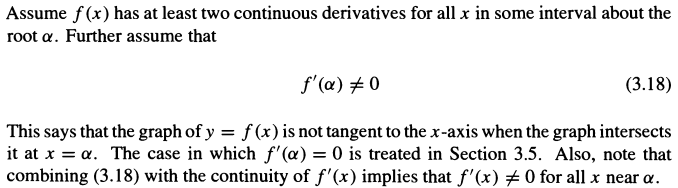
\includegraphics[scale=0.8]{Figures/4}
\end{figure}

\begin{figure}[h!]
	\centering
	
\includegraphics[scale=0.8]{Figures/5}
\end{figure}

\newpage 
%
\begin{exa}
We consider again the first example above.
%
\begin{figure}[h!]
	\centering
	
\includegraphics[scale=0.8]{Figures/6}
\end{figure}
\end{exa}
%
If we assume that the iterate $x_n$ is near the root $\a$, the multiplier on the right of (3.19) can be written as 
\begin{figure}[h!]
	\centering
	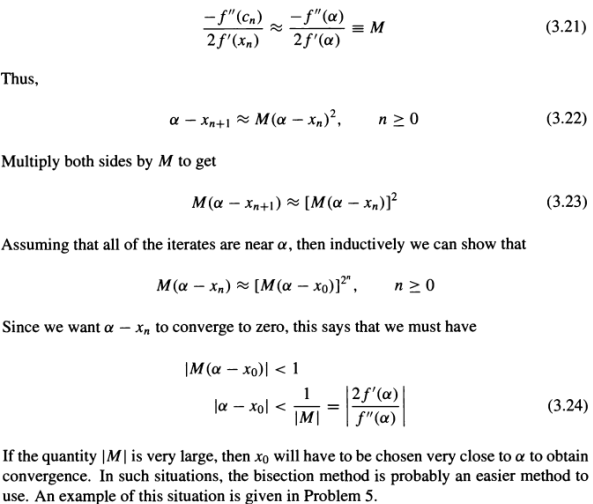
\includegraphics[scale=0.85]{Figures/7}
\end{figure}

\begin{shaded}
The choice of $x_0$ can be very important in determining whether Newton’s method will converge. Unfortunately, there is no single strategy that is always effective in choosing $x_0$. In most instances, a choice of xo arises from the physical situation that led to the rootfinding problem. In other instances, graphing $y=f(x)$ will probably be needed, possibly combined with the bisection method for a few iterates. 
\end{shaded}

\begin{figure}[h!]
	\centering
	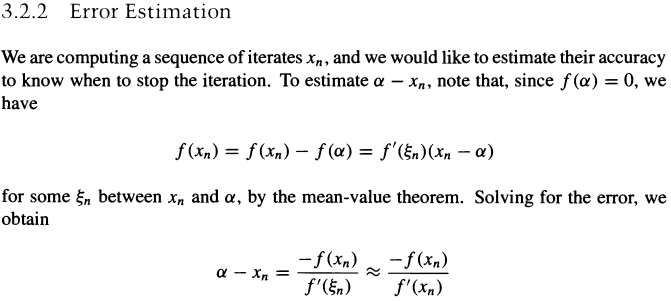
\includegraphics[scale=0.8]{Figures/8}
\end{figure}

\begin{figure}[h!]
	\centering
	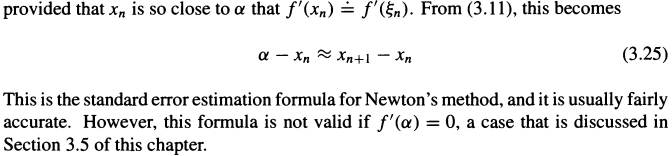
\includegraphics[scale=0.8]{Figures/9}
\end{figure}

\subsection{Extra reading}
In the use of Newton’s method, consideration must be given to the proper choice of a starting point. Usually, onemust have some insight into the shape of the graph of thefunction.Sometimes a coarse graph is adequate, but in other cases, a step-by-step evaluation of the function at various points may be necessary to find a point near the root. Often several steps of the bisection method is used initially to obtain a suitable starting point, and Newton’s method is used to improve the precision. Although Newton’s method is truly a marvelous invention, its convergence depends upon hypotheses that are difficult to verify a priori. Some graphical examples will show what can happen. 

\begin{figure}[h!]
	\centering
	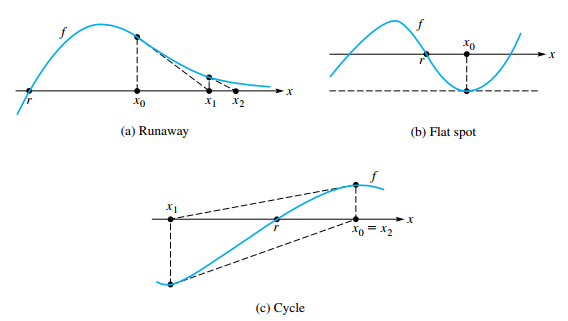
\includegraphics[scale=0.8]{Figures/screenshot0017}
	\caption{Failure of Newton’s method due to bad starting points}
	\label{fig:screenshot0017}
\end{figure}

In Figure \ref{fig:screenshot0017}(a), the tangent to the graph of the function f at $x_0$ intersects the x-axis at a point remote from the root r, and successive points in Newton’s iteration recede from r instead of converging to r. The difficulty can be ascribed to a poor choice of the initial
point $x_0$; it is not sufficiently close to $r$. In Figure \ref{fig:screenshot0017}(b), the tangent to the curve is parallel to the $x$-axis and $x_1 = \pm \infty$, or it is assigned the value of machine infinity in a computer. In Figure \ref{fig:screenshot0017}(c), the iteration values cycle because $x_2 = x_0$. In a computer, roundoff errors or limited precision may eventually cause this situation to become unbalanced such that the iterates either spiral inward and converge or spiral outward and diverge. The analysis that establishes the quadratic convergence discloses another troublesome hypothesis; namely, $f'(r)\neq 0$. 
%
\begin{shaded}
If $f'(r)=0$, then $r$ is a zero of $f$ and $f'$. Such a zero is termed a multiple zero of $f$. In this case, at least a double zero. Newton’s iteration for a multiple zero converges only linearly! Ordinarily, one would not know in advance that the zero sought was a multiple zero. If one knew that the multiplicity was $m$, however, Newton’s
method could be accelerated by modifying the equation to read 
%
\[ x_{n+1} = x_n - m \cfrac{f(x_n)}{f'(x_n)} \]
%
in which $m$ is the multiplicity of the zero in question. 
\end{shaded}
%
\begin{figure}[h!]
	\centering
	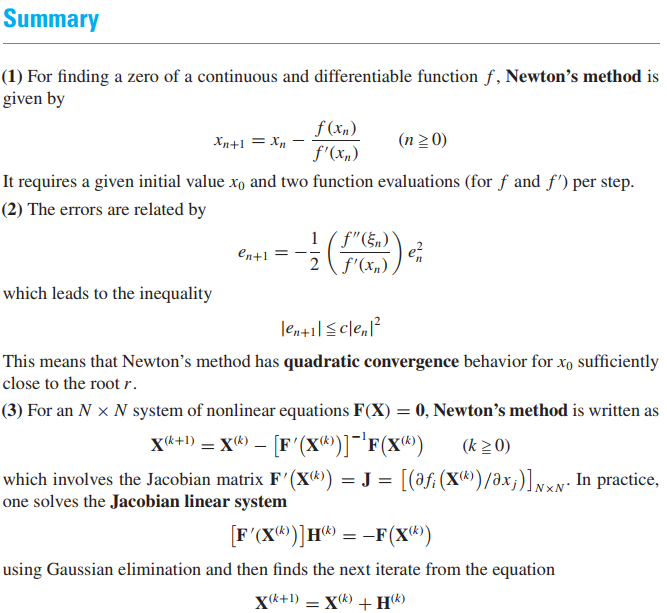
\includegraphics[scale=0.8]{Figures/10}
\end{figure}

\cleardoublepage

\section{Secant method}

In analog to Newton method, the secant method can be viewed from two different perspectives, geometrical and analytical.

\textbf{Geometrical}
\begin{figure}[h!]
	\centering
	
\includegraphics[scale = 0.8]{Figures/11}
	\caption{A geometrical schematic of the secant method: left $x_1<\a< x_0$ and right $\a<x_1<x_0$.}
	\label{fig:11}
\end{figure}

\textbf{Analytical} \ From Newton's method
%
\begin{equation*}
 x_{n+1} = x_n - \cfrac{f(x_n)}{f'(x_n)} \ \mathbf{\approx x_n - f(x_n) \ \cfrac{x_n-x_{n-1}}{f(x_n)-f(x_{n-1})} } \ .
\end{equation*}
%
Notice that, first secant method requires two initial values $x_0$ and $x_1$. After the first step, only one new function evaluation per step is needed.

\subsection{Error analysis}
After $n+1$ steps of the secant method, the error iterates $e_i = \a - x_i$ obey the equation
%
\begin{equation*}
e_{n+1} = - \cfrac{1}{2} \cfrac{f"(\xi_n)}{f'(\zeta_n)} \ e_{n} \ e_{n-1}.
\end{equation*}
%
which leads to the approximation
%
\begin{equation*}
 |e_{n+1}| \approx C|e_n|^{1/2(1+\sqrt{5})} \approx C|e_n|^{1.62} \ .
\end{equation*}
%
Therefore, the secant method has \textbf{superlinear convergence} behavior.

\cleardoublepage

\section{Comparison of Methods}
In this chapter, three primary methods for solving an equation $f(x)=0$ have been presented. The bisection method is reliable but slow. Newton’s method is fast but often only near the root and requires $f'$. The secant method is nearly as fast as Newton’s method and does not require knowledge of the derivative $f'$, which may not be available or may be too expensive to compute. The user of the bisection method must provide two points at which the signs of $f(x)$ differ, and the function f need only be continuous. In using Newton’s method, one must specify a starting point near the root, and f must be differentiable. The secant method requires two good starting points. Newton’s procedure can be interpreted as the repetition of a two-step procedure summarized by the prescription linearize and solve. This strategy is applicable in many other numerical problems, and its importance cannot be overemphasized. Both Newton’s method and the secant method fail to bracket a root. The modified false position method can retain the advantages of both methods. The secant method is often faster at approximating roots of nonlinear functions in comparison to bisection and false position. Unlike these two methods, the intervals $[a_k, b_k]$ do not have to be on opposite sides of the root and have a change of sign. Moreover, the slope of the secant line can become quite small, and a step can move far from the current point. The secant method can fail to find a root of a nonlinear function that has a small slope near the root because the secant line can jump a large amount. For nice functions and guesses relatively close to the root, most of these methods require relatively few iterations before coming close to the root. However, there are pathological functions that can cause troubles for any of those methods. When selecting a method for solving a given nonlinear problem, one must consider many issues such as what you know about the behavior of the function, an interval $[a,b]$ satisfying $f(a)f(b)<0$, the first derivative of the function, a good initial guess to the desired root, and so on.

\cleardoublepage

\section{Ill behavior}

\newpage

\nocite{*}

\bibliography{GTS_reference} 

\end{document}